\chapter{Design}
In this chapter, the design of the prototype and the graphical decisions that were made, will be discussed and defined with the requirements set in the analysis, which were further defined in  design requirements section \ref{DesignRequirements}. When designing, different aspects will be taken into consideration for user experience; usability goals and principles as well as mobile usability (section \ref{Usability}) and  establishing intuition through familiarity. The user experience also depends on the technical implementation of the graphical user interface and non-traditional sensors, while also ensuring that the system performance is smooth. In further design iterations users would be involved in the design process , as user centred design is one of the elements to designing a good user experience (see section \ref{UXUserCentred}).
\section{Concept}
The goal of the prototype is to answer which of the control schemes is the most familiar and efficient when navigating in a 3D virtual environment. Designing this kind of prototype which is not traditional can go in various directions. The concept was then narrowed down to just being multi-touch and using the gyroscope.
The prototype has to implement two features to navigate in a 3D virtual environment. The moving of the camera and the camera rotation. The familiarity concept will be put into effect as the control schemes for controlling the camera have to be linked with something that the user might be familiar with already. 

\section{Interface Design}
The currently existing sensors in mobiles enable the creation of unusual ways of controlling a 3D environment. With the goal in mind of achieving familiarity through the non-traditional sensors, two different approaches were established. The first approach uses the knowledge and familiarity of the current existing products ( see section \ref{SOTA}). The second approach is representing movements related to the ones in real life. For both approaches, the current and the target knowledge (see figure \ref{fig:Knowledge}) is expected to be separate. The design needs to be established in a way that will help the users get through the knowledge gap intuitively, when they are using the interface. It was important to keep the same movement speed settings for all the control schemes for later evaluation. That meant that in the perfect scenario, the user should be able to get from one position to another, with the same amount of time spent for each of the control schemes.

\section{Control Schemes}
Three distinct control schemes were designed for the navigation (see fig. \ref{fig:ControlSchemes}). Buttons-only (fig. \ref{fig:buttonSketch}), Joystick-only ( fig. \ref{fig:joystickSketch}) and one that includes buttons for moving back and forth with a gyroscope for rotating the camera (fig. \ref{fig:gyroSketch}). The fact that newer smart devices are capable of multi-touch input, has been used to enable both the movement and the rotation to be controlled simultaneously. That creates the possibility for the user to walk and turn around at the same time.

\begin{figure}[H]
\centering
  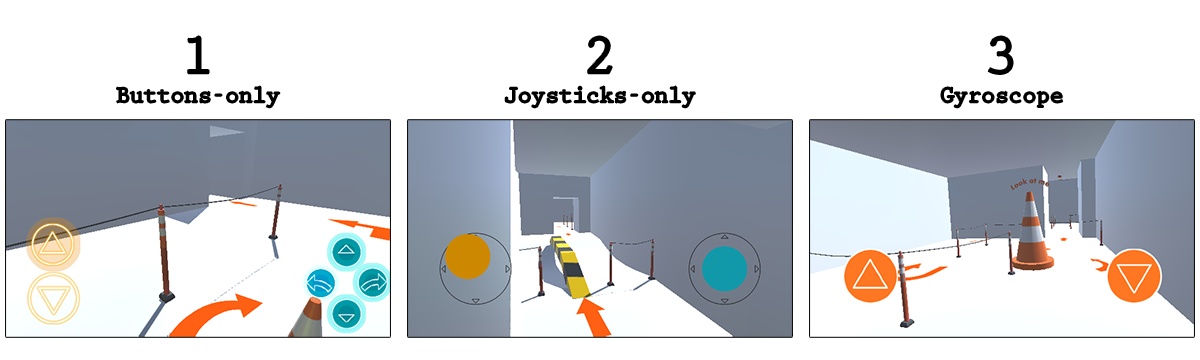
\includegraphics[width=.9\linewidth]{ControlSchemes.png}
  \captionof{figure}{Control Schemes}
  \label{fig:ControlSchemes}
\end{figure}

\subsection{Gyroscopic Controls}
Using the gyroscopic sensor creates the possibility to interact in an unusual but familiar way. It enables the prototype to be built around what is most familiar to movement in real life,  actually turning around in reality to navigate.
Controlling the camera with a built-in gyroscope in the tablet is familiar because it is a natural way for a person to look around. The forward and backward movements were implemented with  buttons, as these were familiar to the target group through the usual human-computer interaction. Most of the controllers for movement are represented as arrows on a computer keyboard, music player or cell phone.
Such control schemes may have the potential to engage the user in the task the most, if the user reaches a state of flow (see page \pageref{FlowTheory}).

\begin{figure}[H]
\centering
\begin{minipage}{.5\textwidth}
  \centering
  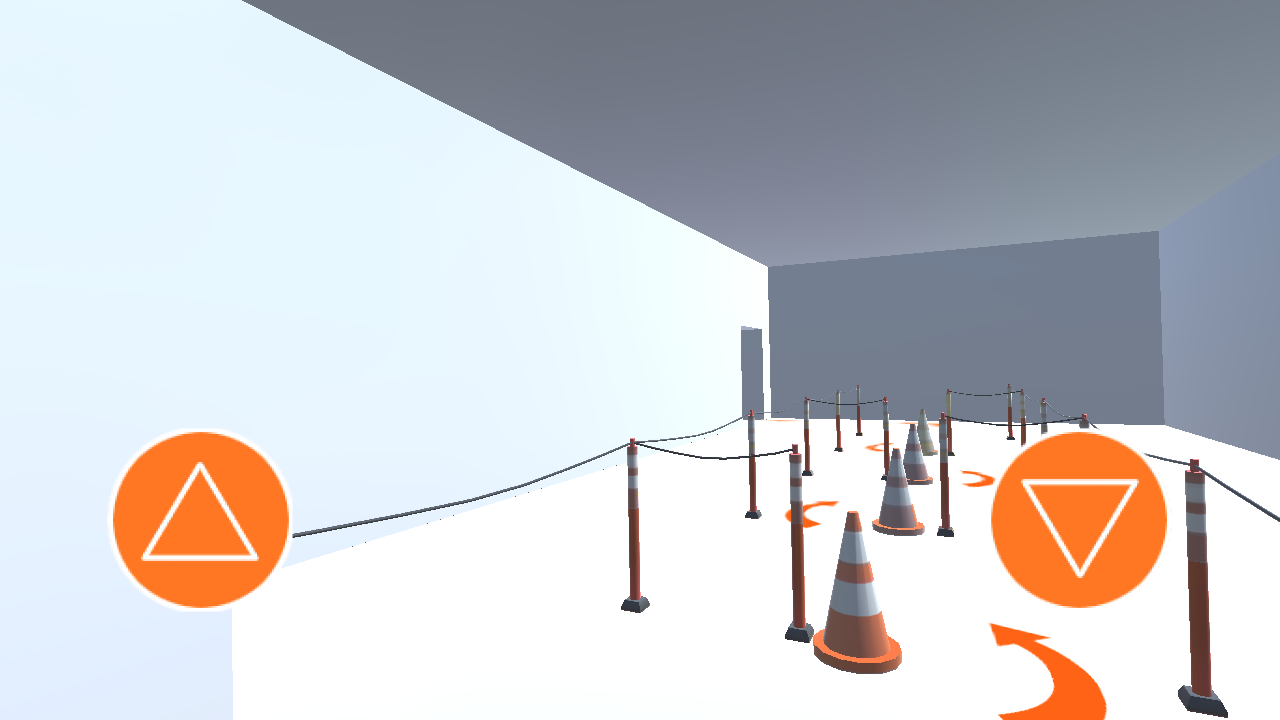
\includegraphics[width=.7\linewidth]{gyro1.png}
\end{minipage}%
\begin{minipage}{.5\textwidth}
  \centering
  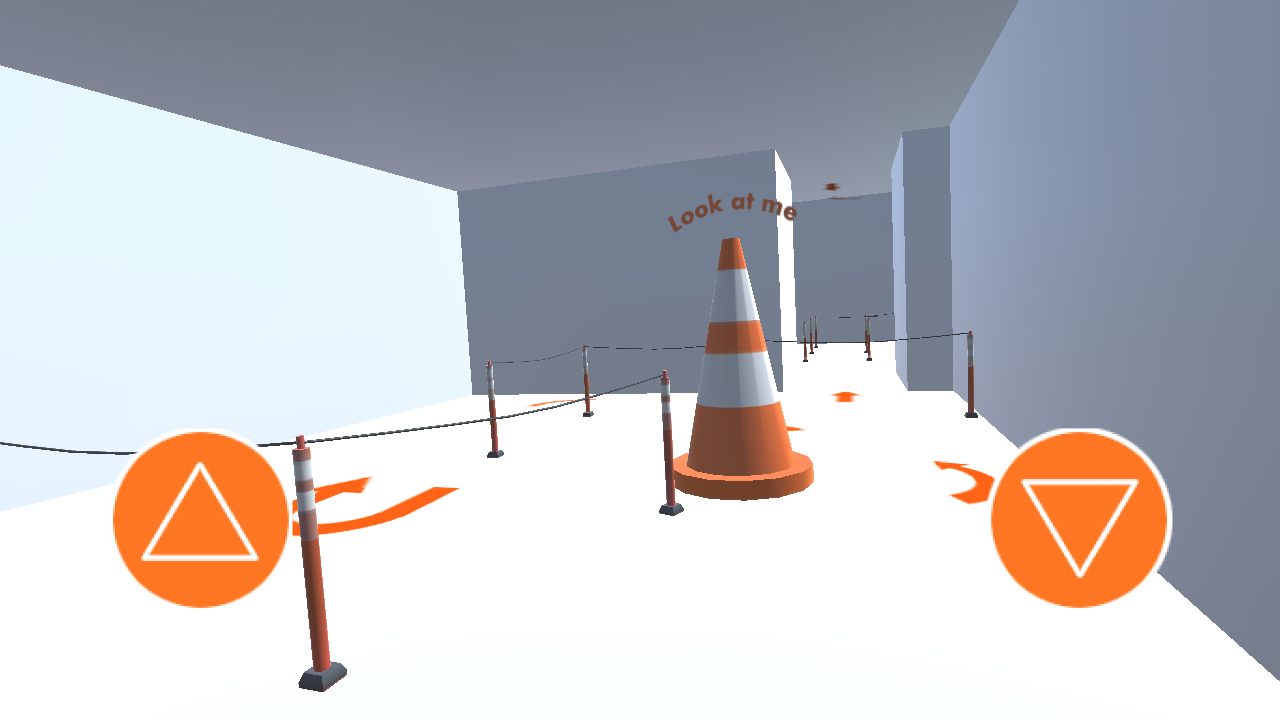
\includegraphics[width=.7\linewidth]{gyro2.png}
\end{minipage}
  \captionof{figure}{Initial sketch of gyroscope}
  \label{fig:gyroSketch}

\end{figure}


\subsection{Joystick}
In this prototype the user has to navigate using two joysticks, one for movement and one for the camera rotation. This should be easy to learn for the users who have used a joystick before. The target group is expected to have some knowledge of how a joystick works. Because of the popularity in games where joysticks are placed on game console's remote controls, like the Sony Playstation or Microsoft Xbox. Even for users with no previous joystick controller experience, this should not be a problem. The control scheme is supposed to borrow the same concept as moving a computer mouse on the screen, both uses 2D directional movement\cite{JRaskin}.

\begin{figure}[H]
\centering
\begin{minipage}{.5\textwidth}
  \centering
  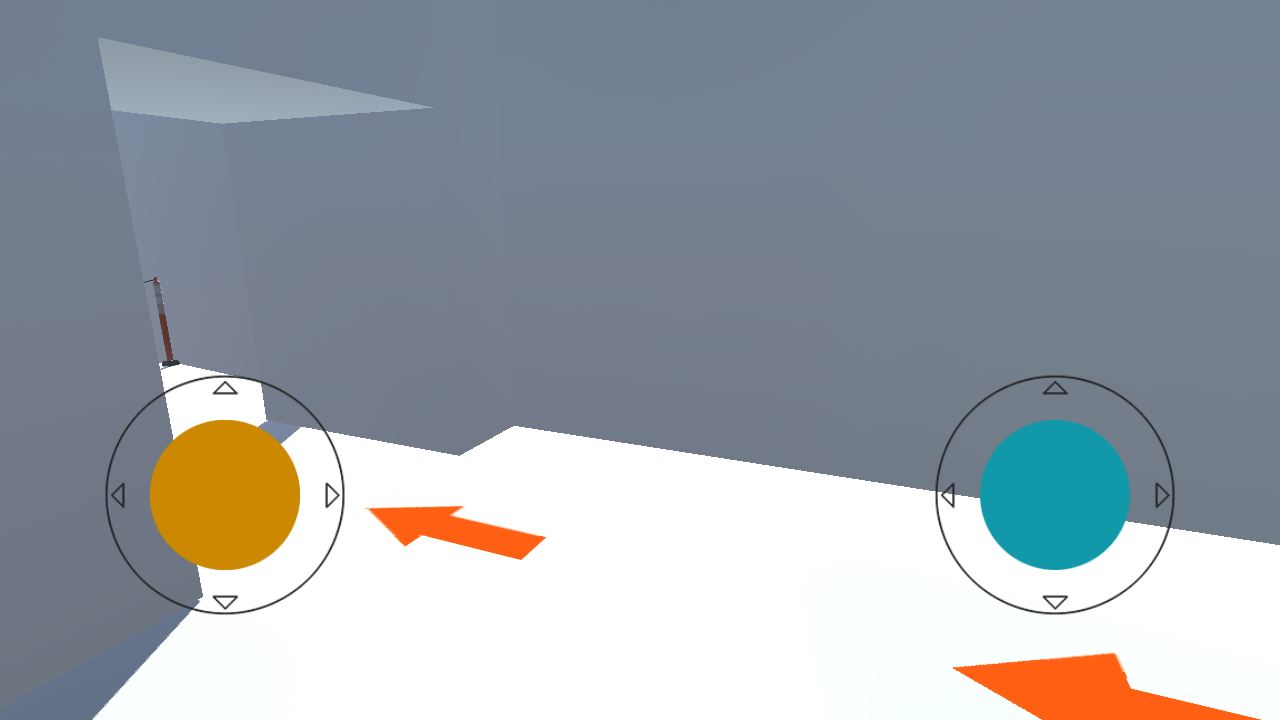
\includegraphics[width=.7\linewidth]{joystick1.png}
\end{minipage}%
\begin{minipage}{.5\textwidth}
  \centering
  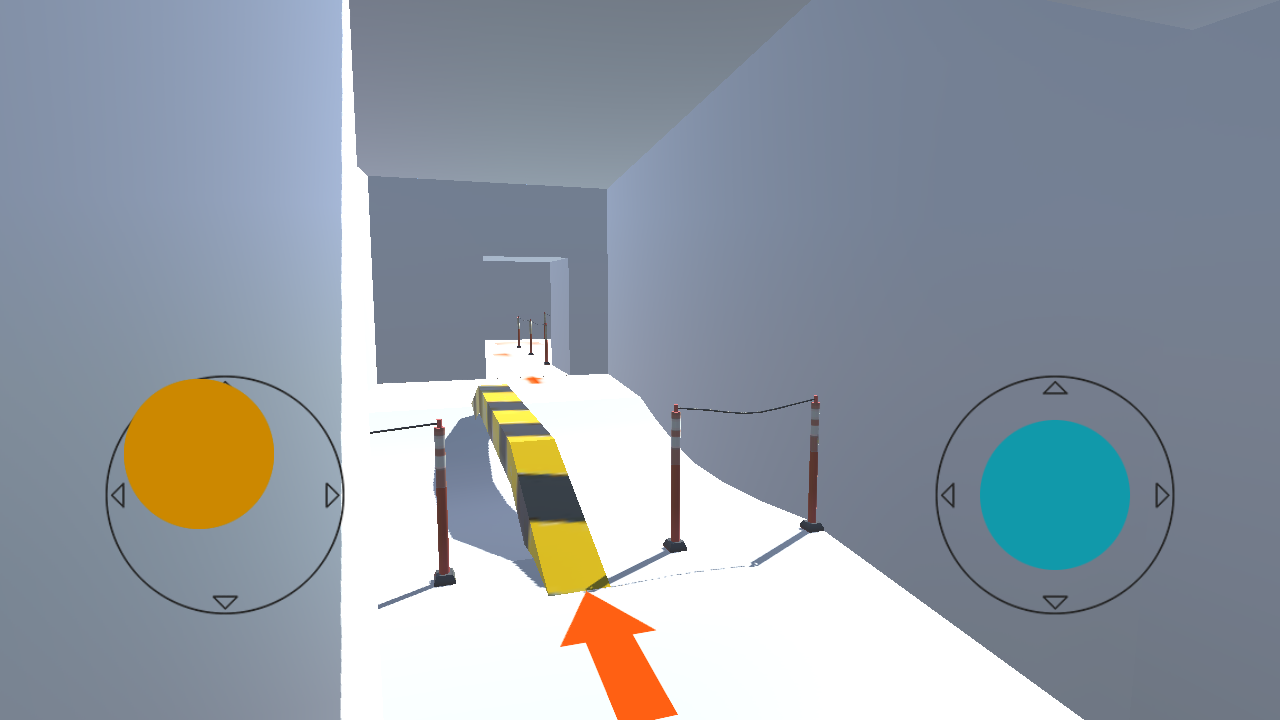
\includegraphics[width=.7\linewidth]{joystick2.png}
\end{minipage}
  \captionof{figure}{Initial sketch of joystick}
  \label{fig:joystickSketch}

\end{figure}

\subsection{On-screen Buttons}
This control scheme is the one that should be the most familiar to the users through daily use. Only using buttons as the way to move both camera and the character. in this case the navigation would only consist of arrow keys located on the screen. This should be familiar to anyone that has used buttons. 

\begin{figure}[H]
\centering
\begin{minipage}{.5\textwidth}
  \centering
  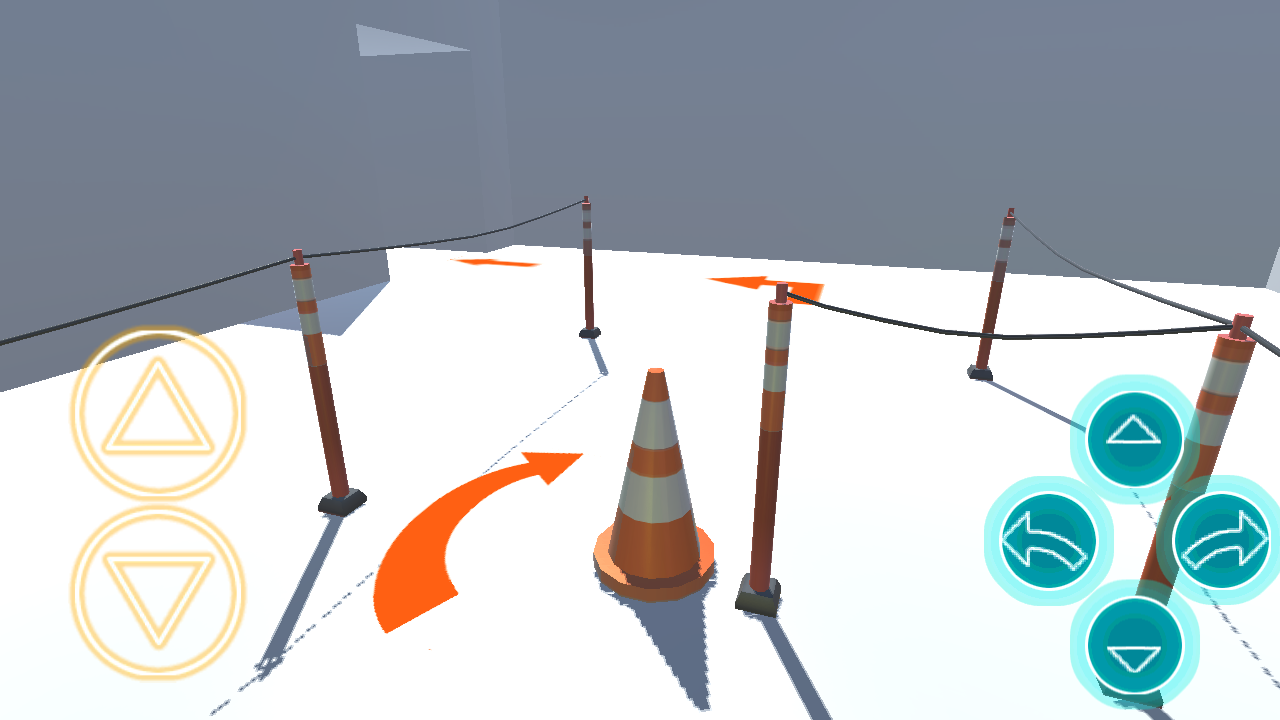
\includegraphics[width=.7\linewidth]{buttons1.png}
\end{minipage}%
\begin{minipage}{.5\textwidth}
  \centering
  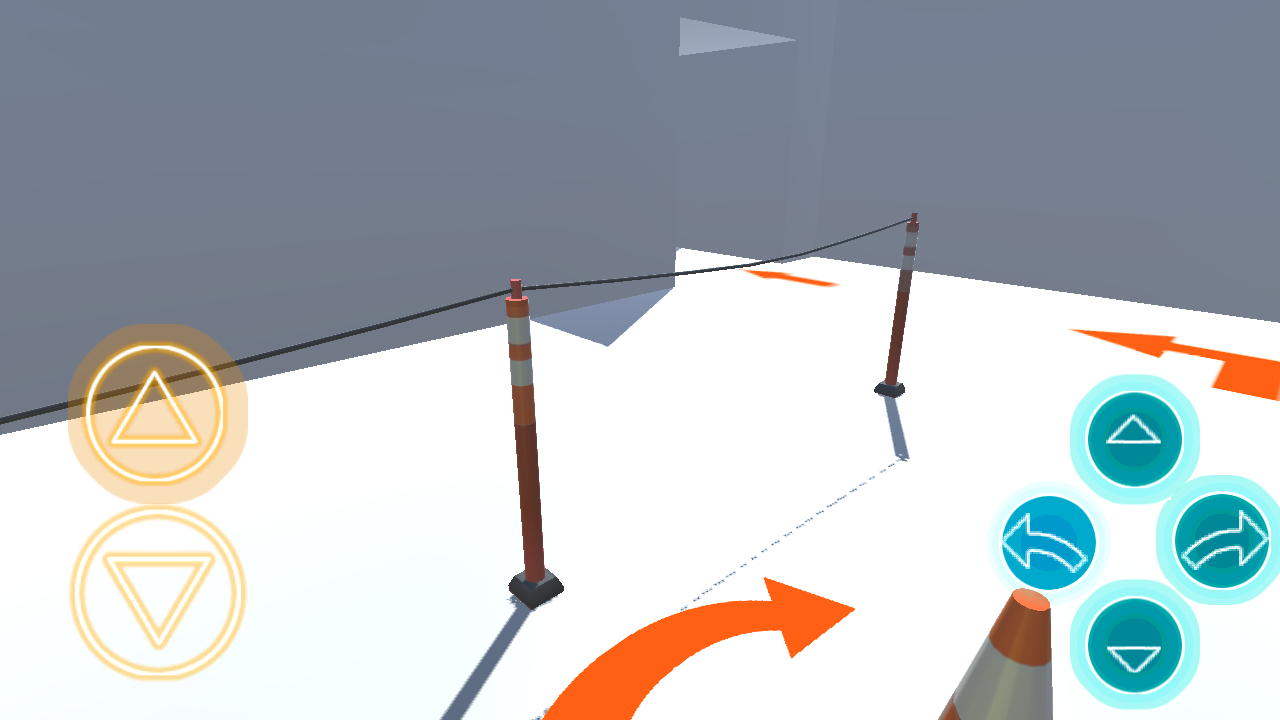
\includegraphics[width=.7\linewidth]{buttons2.png}
\end{minipage}
  \captionof{figure}{Initial sketch of buttons}
  \label{fig:buttonSketch}
\end{figure}

\section{Isolation}
To further emphasize on the initial design requirements, the concept of isolation (see fig. \ref{isolationFig}) should be used when designing the controllers. This is done by making them stand out from the level content. This is supposed to help the user understand what parts of the application gives feedback upon interaction.

\section{Immediacy and Simplicity}
To communicate information faster and simpler, the designs should be represented by concepts that are already familiar to the user. This means, that to communicate information to the user, graphical elements should be represented as symbols that indicate either movement or rotation for the buttons. At the same time it emphasizes the concept of affordance (see section \ref{Usability}), as the buttons represent mechanical buttons, as used in traditional types of controllers. This will further shape the intuition and familiarity for the application

\begin{figure}[H]
\centering
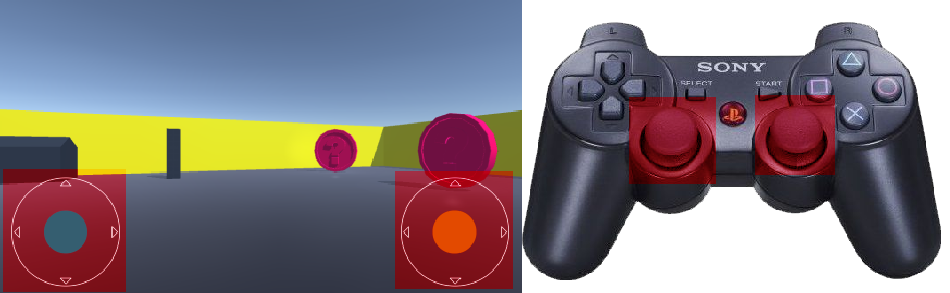
\includegraphics[scale=0.45]{JoystickComparison.png}
\caption{Comparison of initial design sketch of on-screen joystick and the Sony Playstation controller.}
\end{figure}

\section{Graphical element sizes and placement}
To further emphasize on the user experience, the button size should be set accordingly, to ensure that the users would not have difficulties by unintentionally tapping the wrong section of the controls (see section \ref{MobileUsability}). Individual buttons have to be separated from each other and sized for easy accessibility to reduce the "Fat Finger" problem. To enable a bigger view of the environment horizontally, the application will be built to primarily be viewed when holding the device in landscape mode. Since the device is supposed to be held sideways and by both hands, all of the interaction should be done on the sides of the screen for easy access.
To show the difference between movement and rotation controls, they should be given different looks. Shapes of directional arrows for buttons as well as color indication for both buttons and joystick controls.

\begin{figure}[H]
\centering
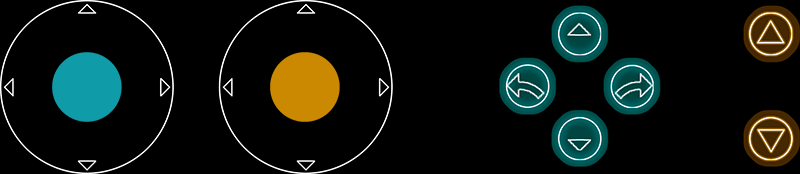
\includegraphics[scale=0.65]{ControllerColors.png}
\caption{Initial sketch. Colour differences to distinguish controllers that hold different functions}
\end{figure}

\section{Design of 3D testing area}\label{DesignTestArea}
To test different non-traditional control schemes a 3D test area was designed. It consists of an obstacle course that test participants have to walk through as fast as possible , see figure\ref{TestLevels}.

\begin{figure}[H]
\centering
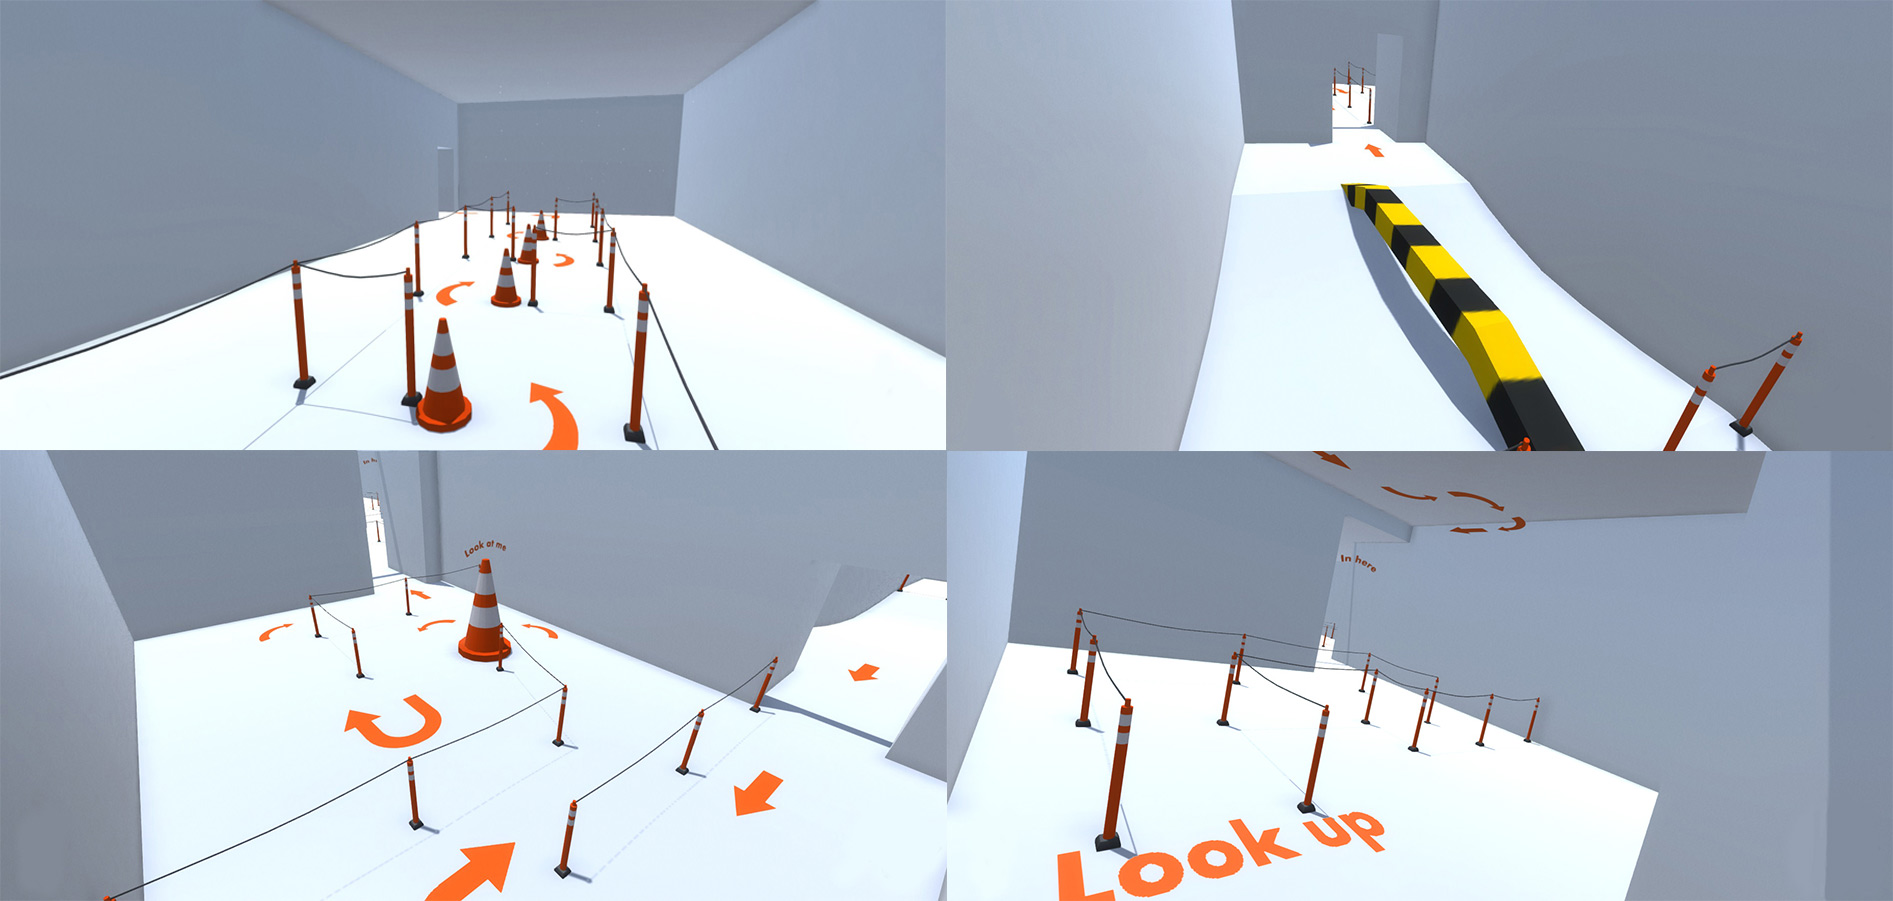
\includegraphics[scale=0.26]{3D_dev_6.jpg}
\caption{Pictures of the testing area}
\label{TestLevels}
\end{figure}

The focus of the testing area was only on navigation. So the tasks and obstacles was in focus and not the environment itself. All non-important bits of the area were coloured a white, neutral colour and important objects as navigational arrows, cones and poles and explanatory text notes, were coloured with a sharp contrasting colour e.g. red and orange. Navigational buttons and important objects in the level were kept in similar colours to help the user recognize and focus on the purpose. 
\section{Design Conclusion}
Three distinct prototypes and a test level was designed for navigation in a 3D environment, with all the initial design requirements in mind. With a goal to create a design that reduces the knowledge gap for the user. These initial prototypes will be implemented as three separate mobile applications for tablets and smartphones. 
In addition, these are not the only possible control schemes that the problem area covers, alternative design possibilities will be discussed in the discussion and redesign chapters later in the report. 